% 03.2. MODELOS DE DATOS
%----------------------------------------------------------------------------------------------
\paragraph{}Nuestro modelo de datos es muy sencillo puesto que solo necesitamos almacenar en la base de datos la información relacionada con los microcontroladores. El resto de la información que manejamos no se almacena en nuestra base de datos; los microcontroladores que introduce un usuario en el carrito de  la compra, los guardamos temporalmente utilizando las funciones de PHP; y la información asociada a un  cliente que realiza una compra, no se almacena en ningún sitio puesto que solo queda reflejada en la factura que se genera cuando se solicita un pedido. \newline

\noindent Por lo tanto, nuestro modelo de datos es el siguiente:

\begin{figure}[h!]
\centering
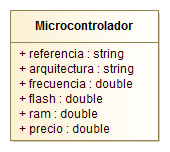
\includegraphics[width=0.40\textwidth]{img/modelo_datos}
\caption{Modelo de datos}
 \label{fig:modelo_datos}
\end{figure}
